%% Version 4.3.2, 25 August 2014
%
%%%%%%%%%%%%%%%%%%%%%%%%%%%%%%%%%%%%%%%%%%%%%%%%%%%%%%%%%%%%%%%%%%%%%%
% Template.tex --  LaTeX-based template for submissions to the 
% American Meteorological Society
%
% Template developed by Amy Hendrickson, 2013, TeXnology Inc., 
% amyh@texnology.com, http://www.texnology.com
% following earlier work by Brian Papa, American Meteorological Society
%
% Email questions to latex@ametsoc.org.
%
%%%%%%%%%%%%%%%%%%%%%%%%%%%%%%%%%%%%%%%%%%%%%%%%%%%%%%%%%%%%%%%%%%%%%
% PREAMBLE
%%%%%%%%%%%%%%%%%%%%%%%%%%%%%%%%%%%%%%%%%%%%%%%%%%%%%%%%%%%%%%%%%%%%%

%% Start with one of the following:
% DOUBLE-SPACED VERSION FOR SUBMISSION TO THE AMS
%\documentclass{ametsoc}

% TWO-COLUMN JOURNAL PAGE LAYOUT---FOR AUTHOR USE ONLY
 \documentclass[twocol]{ametsoc}

%%%%%%%%%%%%%%%%%%%%%%%%%%%%%%%%
%%% To be entered only if twocol option is used

\journal{mwr}

%  Please choose a journal abbreviation to use above from the following list:
% 
%   jamc     (Journal of Applied Meteorology and Climatology)
%   jtech     (Journal of Atmospheric and Oceanic Technology)
%   jhm      (Journal of Hydrometeorology)
%   jpo     (Journal of Physical Oceanography)
%   jas      (Journal of Atmospheric Sciences)	
%   jcli      (Journal of Climate)
%   mwr      (Monthly Weather Review)
%   wcas      (Weather, Climate, and Society)
%   waf       (Weather and Forecasting)
%   bams (Bulletin of the American Meteorological Society)
%   ei    (Earth Interactions)

%%%%%%%%%%%%%%%%%%%%%%%%%%%%%%%%
%Citations should be of the form ``author year''  not ``author, year''
\bibpunct{(}{)}{;}{a}{}{,}

%%%%%%%%%%%%%%%%%%%%%%%%%%%%%%%%

%%% To be entered by author:

%% May use \\ to break lines in title:

\title{Physics-dynamics coupling with Galerkin methods: equal-area physics grid}

%%% Enter authors' names, as you see in this example:
%%% Use \correspondingauthor{} and \thanks{Current Affiliation:...}
%%% immediately following the appropriate author.
%%%
%%% Note that the \correspondingauthor{} command is NECESSARY.
%%% The \thanks{} commands are OPTIONAL.

    %\authors{Author One\correspondingauthor{Author One, 
    % American Meteorological Society, 
    % 45 Beacon St., Boston, MA 02108.}
% and Author Two\thanks{Current affiliation: American Meteorological Society, 
    % 45 Beacon St., Boston, MA 02108.}}

\authors{Peter H. Lauritzen\correspondingauthor{Climate and Global Dynamics, National Center for Atmospheric Research, 1850 Table Mesa Drive, Boulder, Colorado, USA.}}

%% Follow this form:
    % \affiliation{American Meteorological Society, 
    % Boston, Massachusetts.}

\affiliation{Climate and Global Dynamics, National Center for Atmospheric Research, 1850 Table Mesa Drive, Boulder, Colorado, USA.}

%% Follow this form:
    %\email{latex@ametsoc.org}

\email{pel@ucar.edu}

%% If appropriate, add additional authors, different affiliations:
\extraauthor{Mark A. Taylor}
\extraaffil{Sandia National Laboratories, Albuquerque, New Mexico, USA.}
\extraauthor{Paul A. Ullrich}
\extraaffil{Department of Land, Air and Water Resources, University of California, Davis, California, USA}
\extraauthor{Julio T. Bacmeister}
\extraaffil{Climate and Global Dynamics, National Center for Atmospheric Research, 1850 Table Mesa Drive, Boulder, Colorado, USA.}
\extraauthor{Steve Goldhaber}
\extraaffil{Climate and Global Dynamics, National Center for Atmospheric Research, 1850 Table Mesa Drive, Boulder, Colorado, USA.}

%% May repeat for a additional authors/affiliations:

%\extraauthor{}
%\extraaffil{}

%%%%%%%%%%%%%%%%%%%%%%%%%%%%%%%%%%%%%%%%%%%%%%%%%%%%%%%%%%%%%%%%%%%%%
% ABSTRACT
%
% Enter your abstract here
% Abstracts should not exceed 250 words in length!
%
% For BAMS authors only: If your article requires a Capsule Summary, please place the capsule text at the end of your abstract
% and identify it as the capsule. Example: This is the end of the abstract. (Capsule Summary) This is the capsule summary. 

\abstract{Enter the text of your abstract here.}

\begin{document}

%% Necessary!
\maketitle


%%%%%%%%%%%%%%%%%%%%%%%%%%%%%%%%%%%%%%%%%%%%%%%%%%%%%%%%%%%%%%%%%%%%%
% MAIN BODY OF PAPER
%%%%%%%%%%%%%%%%%%%%%%%%%%%%%%%%%%%%%%%%%%%%%%%%%%%%%%%%%%%%%%%%%%%%%
%

%% In all cases, if there is only one entry of this type within
%% the higher level heading, use the star form: 
%%
\section{Introduction}
\begin{itemize}
\item \cite{LH1997MWR}: Believable scales
\item Discuss \cite{W2014PTRSL}: spectral truncation and physics (physical) grid (see page 10; conclusions)
\item \cite{T1999T}: keep physics scales constant with dynamical core refinement in spectral transform model
\begin{itemize}
\item aid the convergence of the Hadley circulation
\item does not convergenge if the physics grid resolution is not held constant
\item parameterizations at the coarser grid do not include their own forcings from the finer scale, which appears to be contradictory to the purpose of parameterizations in the first place.
\end{itemize}
\item \cite{M2009T}: vertical refinement of physics grid (improvement)
\item see complete list of possibly relevant papers in: {\verb+http://pdc.cicese.mx/program_day_by_day.html+}
\end{itemize}

% \subsection*{subsection}
% text...
\section{Methods}
\subsection{Remapping state: GLL grid $\rightarrow$ physics grid}
Requirements for the mapping algorithm:
\begin{itemize}
\item mass-conservative,
\item shape-preserving (monotone),
\item consistent (preserves a constant),
\item preserve basis function order for smooth fields.
\end{itemize}
A possible desirable property is total energy conservation (not pursued here).

In order to achieve conservation of scalar and air mass during the remapping process the constituent mixing ratios are weighted by the pressure level thickness $\Delta p$ before the mapping:
\begin{equation}
\psi=\phi_k\, \Delta p_k,
\end{equation}
where sub-script $k$ refers to the level index. [conversion back]


\begin{figure}[t]
\noindent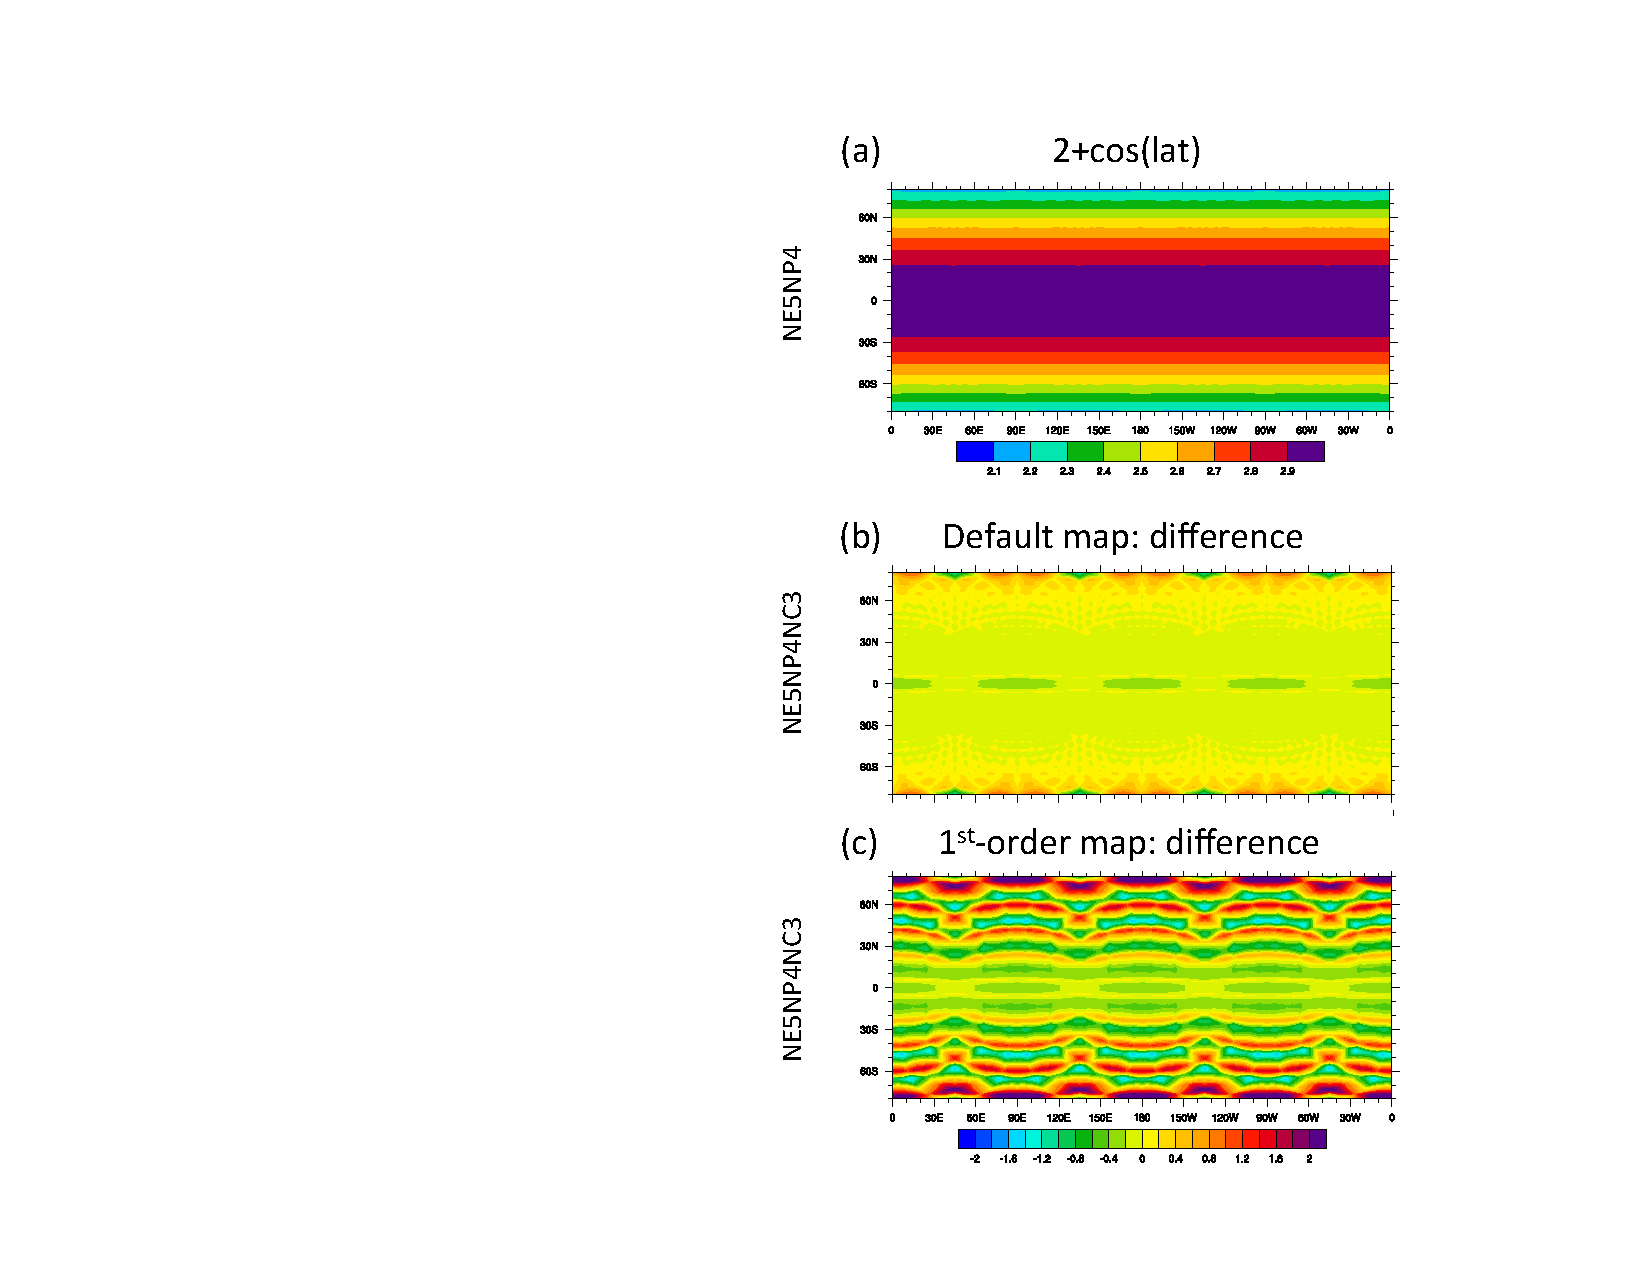
\includegraphics[width=19pc,angle=0]{figs/idealized-mapping-tests-smooth-field.pdf}\\
\caption{(a) Smooth function ($2+\cos(\theta)$) initialized on the $NE5NP4$ GLL grid. (b) and (c) show the difference between the interpolated field and the analytical value at the physics grid cell center. The interpolation is from the $NE5NP4$ GLL grid to the NE5NP4NC3 physics grid (both have an approximate grid spacing of $6^\circ$). In (b) the interpolation algorithm is the default algorithm that is higher-order for smooth fields, shape-preserving, consistent, and mass-conservative. (c) is the same as (b) but using the first-order mapping method. All data has been bilinearly interpolated to a $1^\circ$ regular latitude-longitude grid for plotting.}\label{fig:remap-smooth-field}
\end{figure}
\begin{figure}[t]
\noindent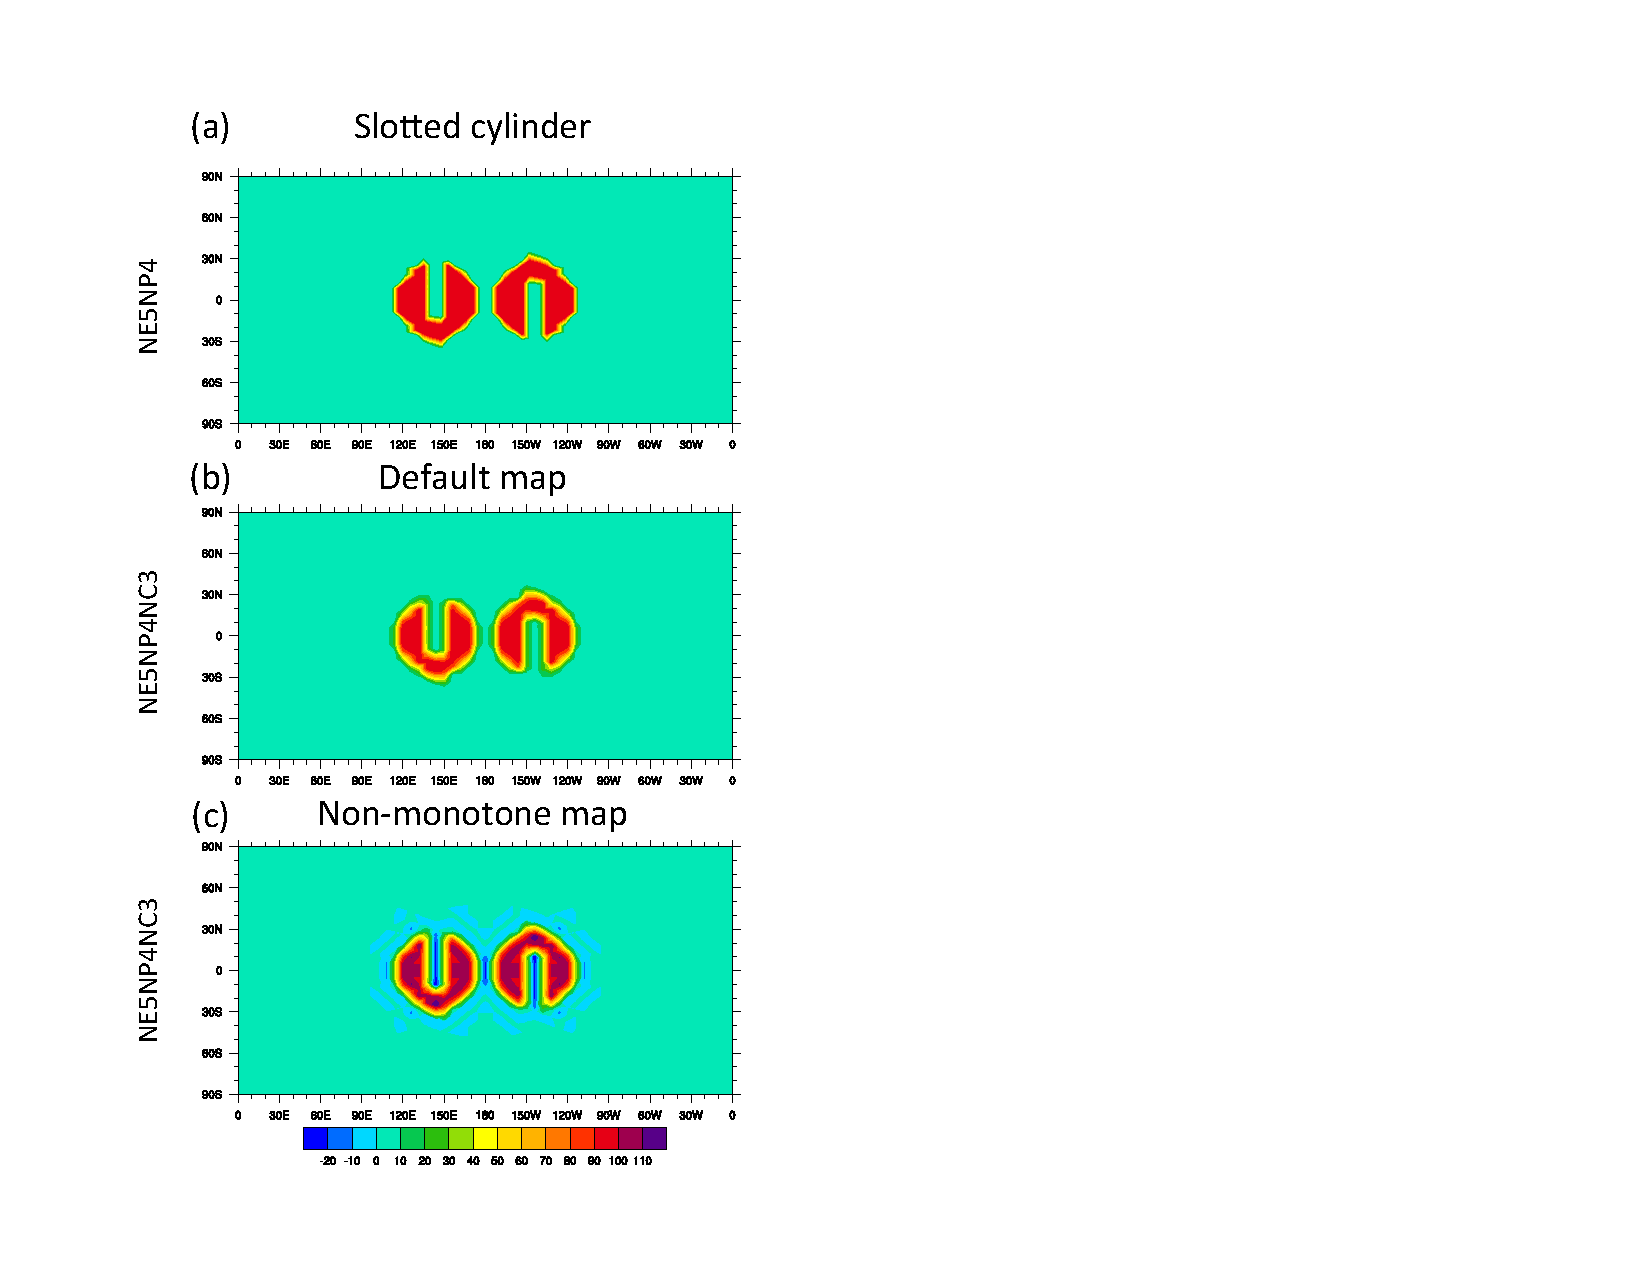
\includegraphics[width=19pc,angle=0]{figs/idealized-mapping-tests-slotted-cylinder.pdf}\\
  \caption{(a) Slotted-cylinder distribution initialized on on the $NE5NP4$ GLL grid (approximately $6^\circ$ resolution). (b) Default mapping of the $NE5NP4$ GLL grid data to the physics grid $NE5NP4NC3$. (c) Same as (b) but using the non-monotone map. All data has been bilinearly interpolated to a $1^\circ\
$ regular latitude-longitude grid for plotting.}\label{fig:remap-slotted-cylinder}
\end{figure}





\subsection{Remapping: physics grid $\rightarrow$ GLL grid}
\section{Results}
\begin{figure}[t]
\noindent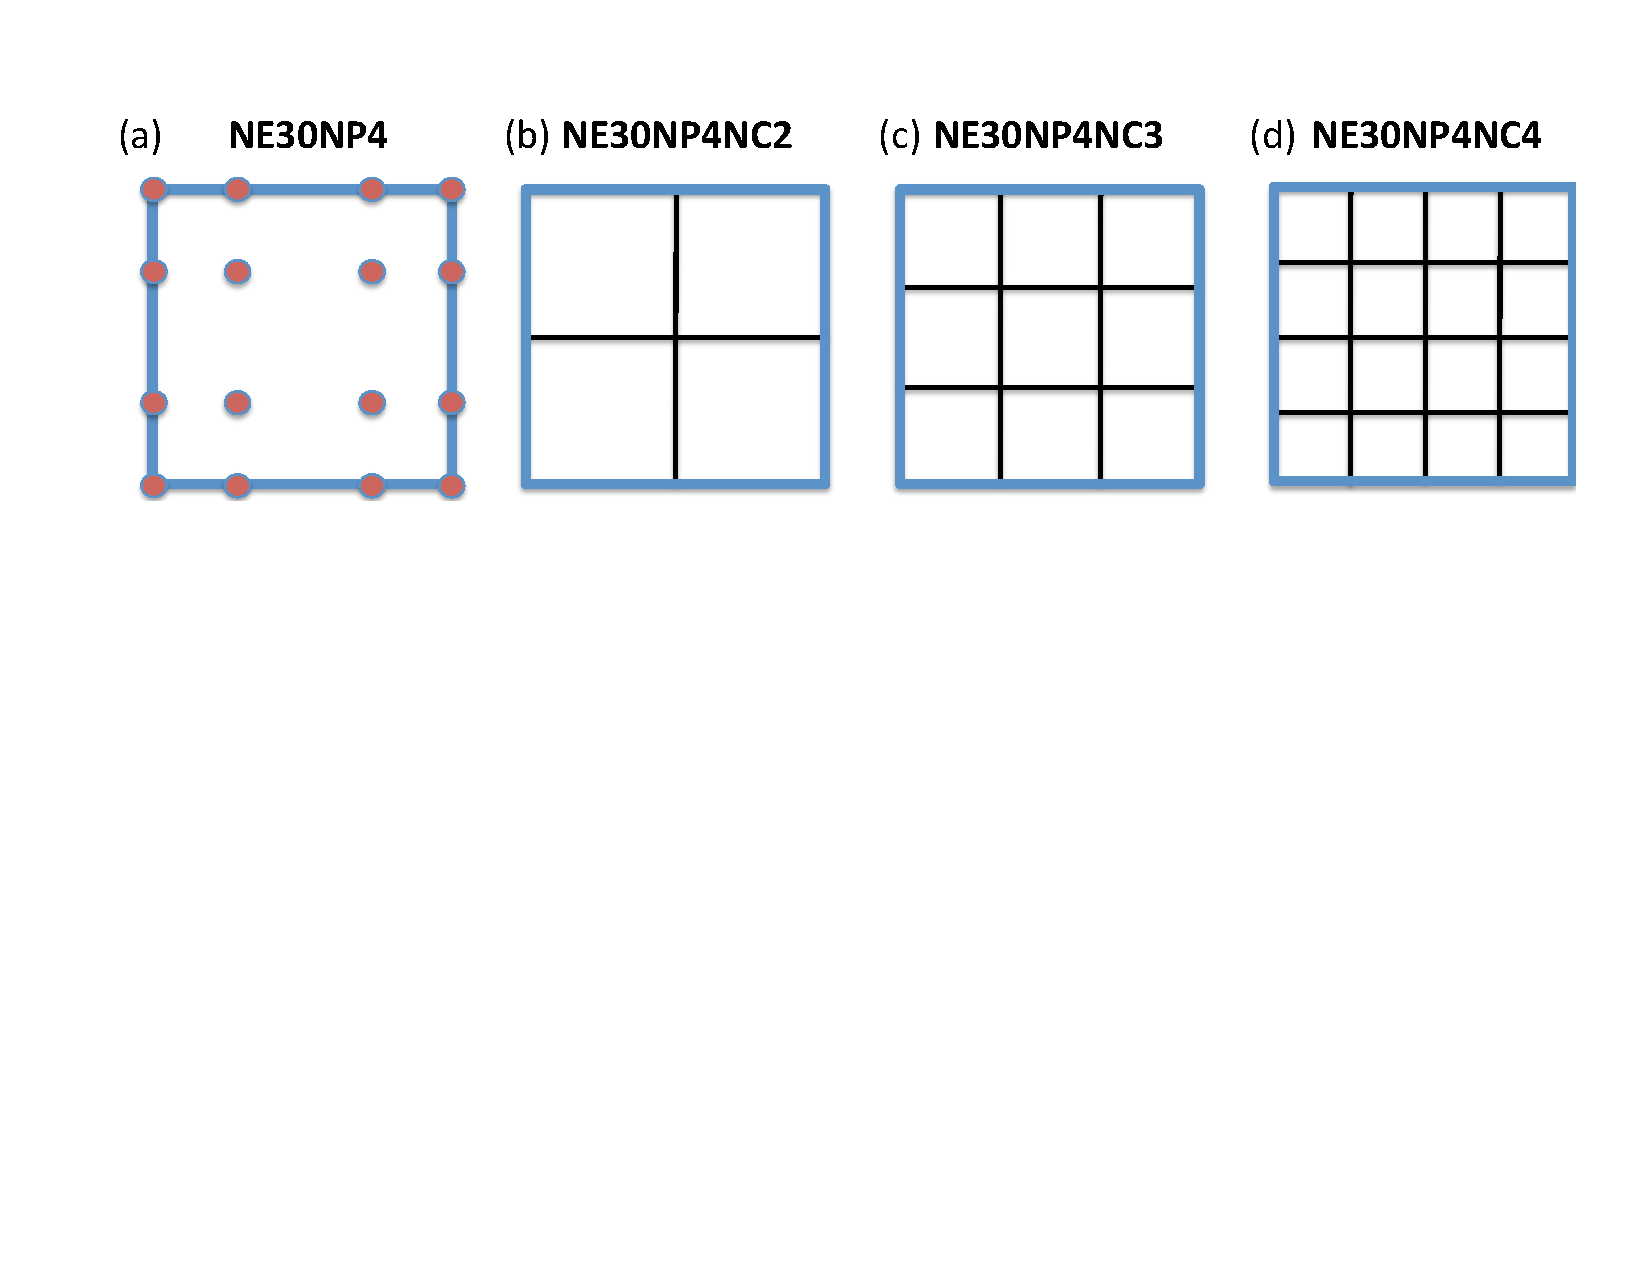
\includegraphics[width=19pc,angle=0]{figs/grids.pdf}\\
  \caption{A graphical illustration of the different physics coloumn configurations: (a) Gauss-Lobatto-Legendre quadrature grid for $np=4$ (filled circles) and (b-d) `equal-area' finite-volume grids of different resolutions ($nc=2,3,4$).}\label{fig:grids}
\end{figure}
%vs

% \section{Section title}
% \subsection{subsection one}
% text...
% \subsection{subsection two}
% \section{Section title}

%%%
\section{Results}
\begin{figure}[t]
\noindent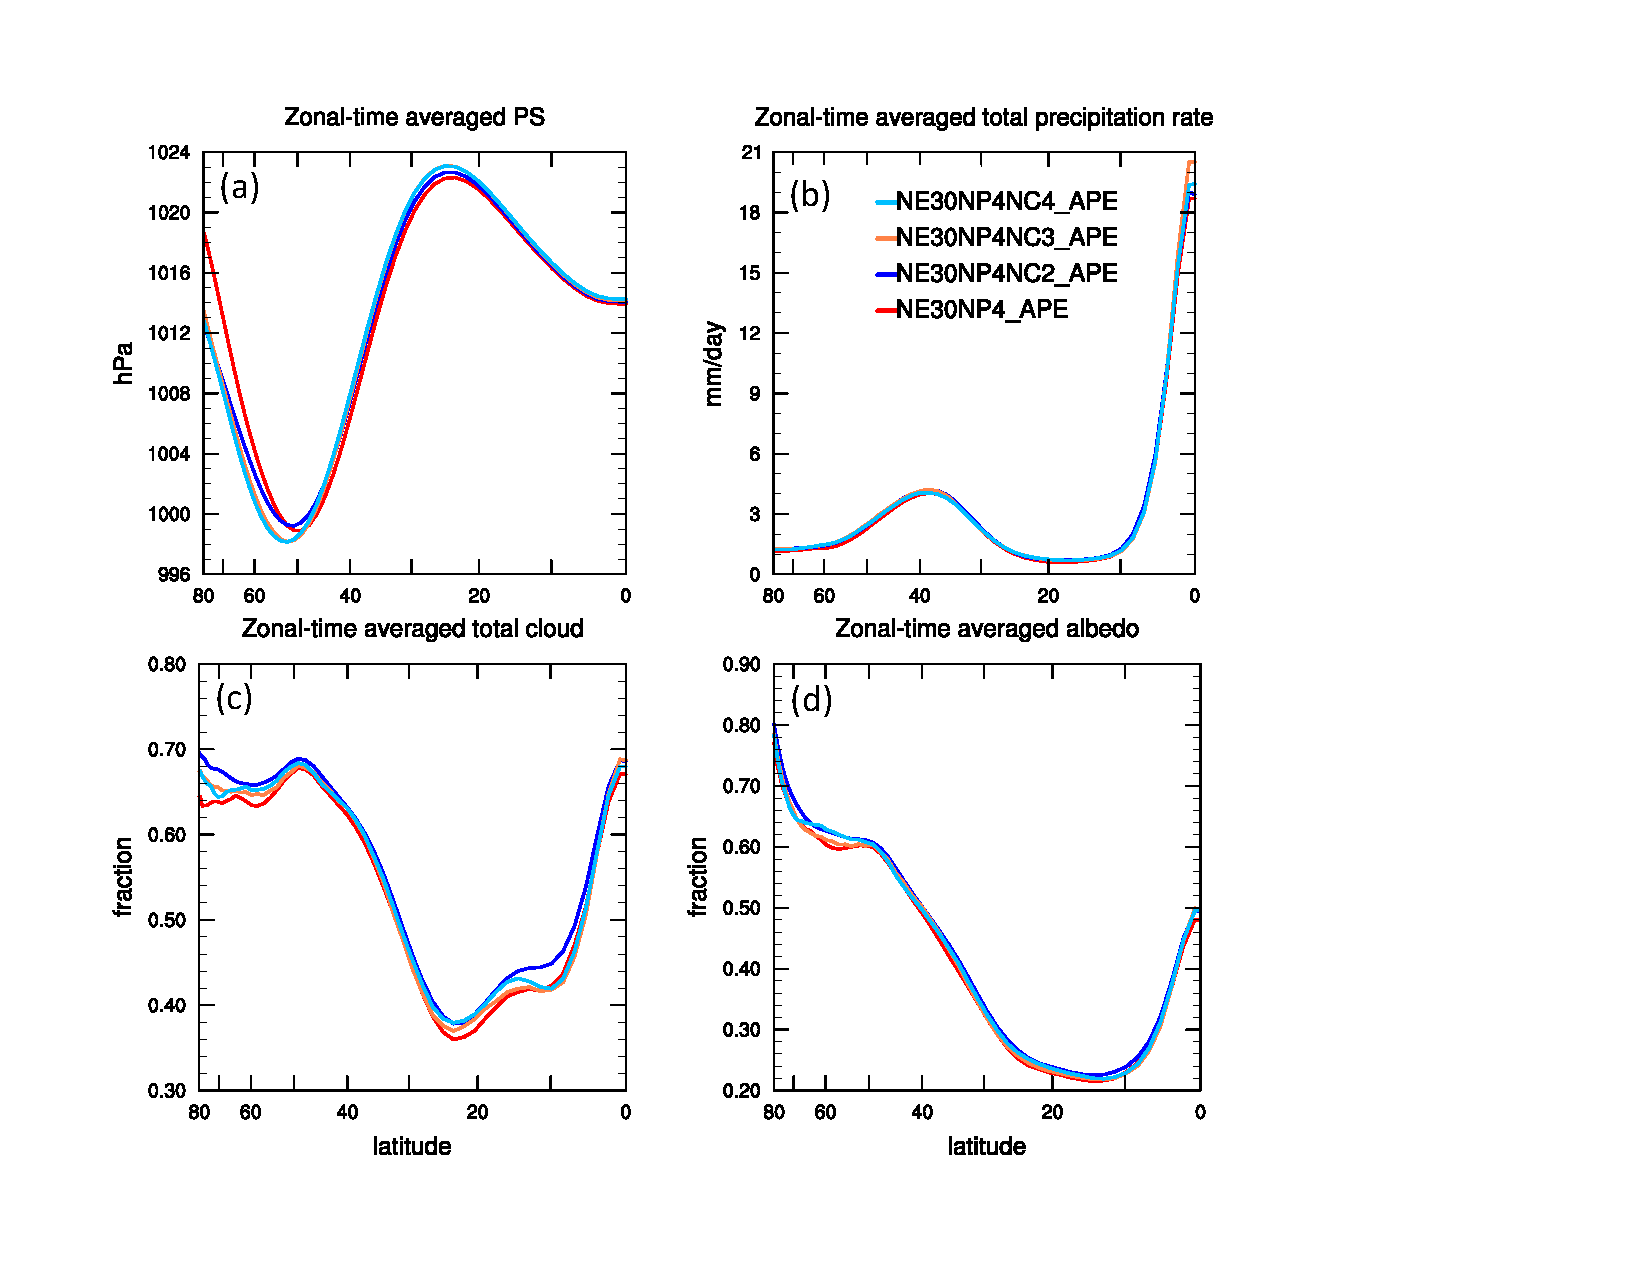
\includegraphics[width=19pc,angle=0]{figs/zonal_time_avg_2d_fields.pdf}\\
\caption{Zonal-time average (a) surface pressure $PS$, (b) total precipitation rate $PRECT$, (c) total cloud fraction $CLDTOT$, and (d) albedo as a function of latitude (from Equator to $80^\circ$N) for the different model configurations. The data has been averaged over a period of 30 months and mapped to a $1.5^\circ$$\times$$1.5^\circ$ regular latitude-longitude grid for analysis.}
\end{figure}

% \subsection{First secondary heading}

% \subsubsection{First tertiary heading}

% \paragraph{First quaternary heading}

%%%%%%%%%%%%%%%%%%%%%%%%%%%%%%%%%%%%%%%%%%%%%%%%%%%%%%%%%%%%%%%%%%%%%
% ACKNOWLEDGMENTS
%%%%%%%%%%%%%%%%%%%%%%%%%%%%%%%%%%%%%%%%%%%%%%%%%%%%%%%%%%%%%%%%%%%%%
%
\acknowledgments
Start acknowledgments here.

%%%%%%%%%%%%%%%%%%%%%%%%%%%%%%%%%%%%%%%%%%%%%%%%%%%%%%%%%%%%%%%%%%%%%
% APPENDIXES
%%%%%%%%%%%%%%%%%%%%%%%%%%%%%%%%%%%%%%%%%%%%%%%%%%%%%%%%%%%%%%%%%%%%%
%
% Use \appendix if there is only one appendix.
%\appendix

% Use \appendix[A], \appendix}[B], if you have multiple appendixes.
%\appendix[A]

%% Appendix title is necessary! For appendix title:
%\appendixtitle{}

%%% Appendix section numbering (note, skip \section and begin with \subsection)
% \subsection{First primary heading}

% \subsubsection{First secondary heading}

% \paragraph{First tertiary heading}

%% Important!
%\appendcaption{<appendix letter and number>}{<caption>} 
%must be used for figures and tables in appendixes, e.g.,
%
%\begin{figure}
%\noindent\includegraphics[width=19pc,angle=0]{figure01.pdf}\\
%\appendcaption{A1}{Caption here.}
%\end{figure}
%
% All appendix figures/tables should be placed in order AFTER the main figures/tables, i.e., tables, appendix tables, figures, appendix figures.
%
%%%%%%%%%%%%%%%%%%%%%%%%%%%%%%%%%%%%%%%%%%%%%%%%%%%%%%%%%%%%%%%%%%%%%
% REFERENCES
%%%%%%%%%%%%%%%%%%%%%%%%%%%%%%%%%%%%%%%%%%%%%%%%%%%%%%%%%%%%%%%%%%%%%
% Make your BibTeX bibliography by using these commands:
\bibliographystyle{ametsoc2014}
\bibliography{bib}


%%%%%%%%%%%%%%%%%%%%%%%%%%%%%%%%%%%%%%%%%%%%%%%%%%%%%%%%%%%%%%%%%%%%%
% TABLES
%%%%%%%%%%%%%%%%%%%%%%%%%%%%%%%%%%%%%%%%%%%%%%%%%%%%%%%%%%%%%%%%%%%%%
%% Enter tables at the end of the document, before figures.
%%
%
%\begin{table}[t]
%\caption{This is a sample table caption and table layout.  Enter as many tables as
%  necessary at the end of your manuscript. Table from Lorenz (1963).}\label{t1}
%\begin{center}
%\begin{tabular}{ccccrrcrc}
%\hline\hline
%$N$ & $X$ & $Y$ & $Z$\\
%\hline
% 0000 & 0000 & 0010 & 0000 \\
% 0005 & 0004 & 0012 & 0000 \\
% 0010 & 0009 & 0020 & 0000 \\
% 0015 & 0016 & 0036 & 0002 \\
% 0020 & 0030 & 0066 & 0007 \\
% 0025 & 0054 & 0115 & 0024 \\
%\hline
%\end{tabular}
%\end{center}
%\end{table}

%%%%%%%%%%%%%%%%%%%%%%%%%%%%%%%%%%%%%%%%%%%%%%%%%%%%%%%%%%%%%%%%%%%%%
% FIGURES
%%%%%%%%%%%%%%%%%%%%%%%%%%%%%%%%%%%%%%%%%%%%%%%%%%%%%%%%%%%%%%%%%%%%%
%% Enter figures at the end of the document, after tables.
%%
%
%\begin{figure}[t]
%  \noindent\includegraphics[width=19pc,angle=0]{figure01.pdf}\\
%  \caption{Enter the caption for your figure here.  Repeat as
%  necessary for each of your figures. Figure from \protect\cite{Knutti2008}.}\label{f1}
%\end{figure}

\end{document}
